\documentclass[11pt,a4paper]{report}
\usepackage[textwidth=37em,vmargin=30mm]{geometry}
\usepackage{calc,xunicode,amsmath,amssymb,paralist,enumitem,tabu,booktabs,datetime2,xeCJK,xeCJKfntef,listings}
\usepackage{tocloft,fancyhdr,tcolorbox,xcolor,graphicx,eso-pic,xltxtra,xelatexemoji}

\newcommand{\envyear}[0]{2025}
\newcommand{\envdatestr}[0]{2025-07-03}
\newcommand{\envfinaldir}[0]{webdb/2025/20250703/final}

\usepackage[hidelinks]{hyperref}
\hypersetup{
    colorlinks=false,
    pdfpagemode=FullScreen,
    pdftitle={Web Digest - \envdatestr}
}

\setlength{\cftbeforechapskip}{10pt}
\renewcommand{\cftchapfont}{\rmfamily\bfseries\large\raggedright}
\setlength{\cftbeforesecskip}{2pt}
\renewcommand{\cftsecfont}{\sffamily\small\raggedright}

\setdefaultleftmargin{2em}{2em}{1em}{1em}{1em}{1em}

\usepackage{xeCJK,xeCJKfntef}
\xeCJKsetup{PunctStyle=plain,RubberPunctSkip=false,CJKglue=\strut\hskip 0pt plus 0.1em minus 0.05em,CJKecglue=\strut\hskip 0.22em plus 0.2em}
\XeTeXlinebreaklocale "zh"
\XeTeXlinebreakskip = 0pt


\setmainfont{Brygada 1918}
\setromanfont{Brygada 1918}
\setsansfont{IBM Plex Sans}
\setmonofont{JetBrains Mono NL}
\setCJKmainfont{Noto Serif CJK SC}
\setCJKromanfont{Noto Serif CJK SC}
\setCJKsansfont{Noto Sans CJK SC}
\setCJKmonofont{Noto Sans CJK SC}

\setlength{\parindent}{0pt}
\setlength{\parskip}{8pt}
\linespread{1.15}

\lstset{
	basicstyle=\ttfamily\footnotesize,
	numbersep=5pt,
	backgroundcolor=\color{black!5},
	showspaces=false,
	showstringspaces=false,
	showtabs=false,
	tabsize=2,
	captionpos=b,
	breaklines=true,
	breakatwhitespace=true,
	breakautoindent=true,
	linewidth=\textwidth
}






\newcommand{\coverpic}[2]{
    % argv: itemurl, authorname
    Cover photo by #2~~(\href{#1}{#1})
}
\newcommand{\makeheader}[0]{
    \begin{titlepage}
        % \newgeometry{hmargin=15mm,tmargin=21mm,bmargin=12mm}
        \begin{center}
            
            \rmfamily\scshape
            \fontspec{BaskervilleF}
            \fontspec{Old Standard}
            \fontsize{59pt}{70pt}\selectfont
            WEB\hfill DIGEST
            
            \vfill
            % \vskip 30pt
            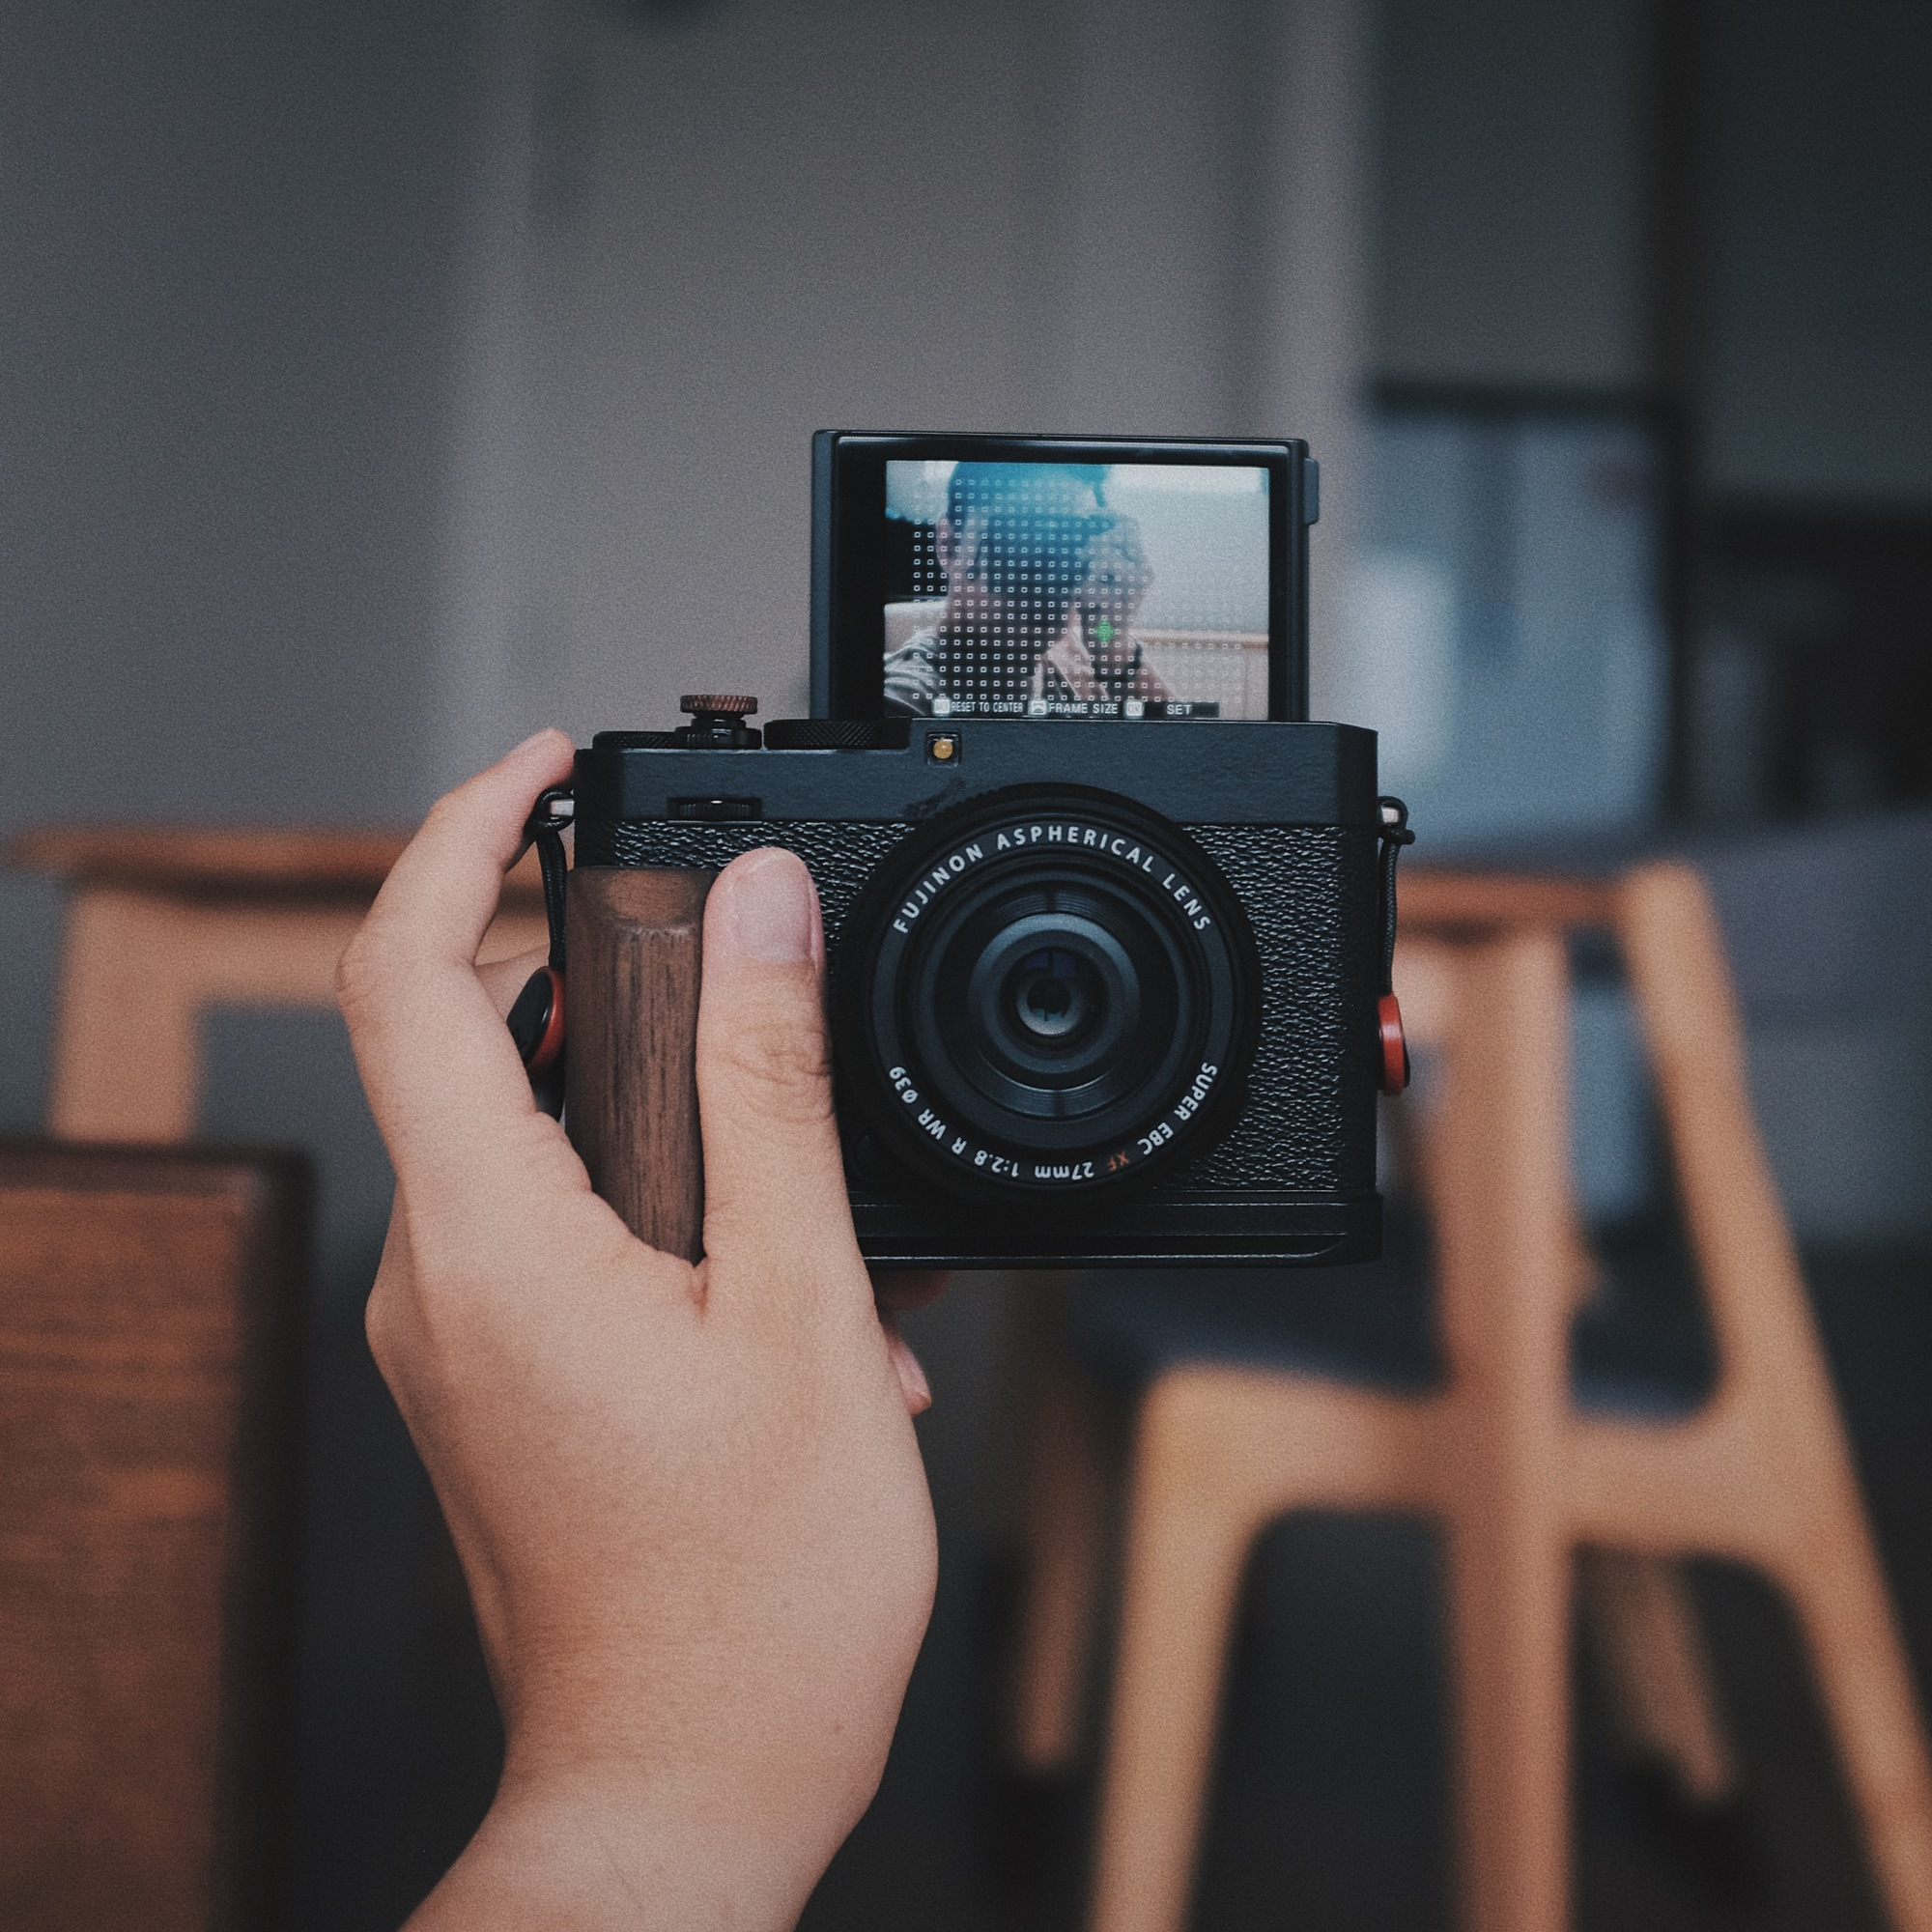
\includegraphics[width=\linewidth]{\envfinaldir/coverpic-prod.jpg}\par
            % \vskip 30pt
            \vfill

            \normalsize\rmfamily\scshape
            \copyright{} The Web Digest Project \hfill\large \envdatestr
        \end{center}
    \end{titlepage}
    % \restoregeometry
}
\newcommand{\simplehref}[1]{%
    \textcolor{blue!80!green}{\href{#1}{#1}}%
}
\renewcommand{\contentsname}{\center\Huge\sffamily\bfseries Contents\par\vskip 20pt}
\newcounter{ipartcounter}
\setcounter{ipartcounter}{0}
\newcommand{\ipart}[1]{
    % \vskip 20pt
    \clearpage
    \stepcounter{ipartcounter}
    \phantomsection
    \addcontentsline{toc}{chapter}{#1}
    % \begin{center}
    %     \Huge
    %     \sffamily\bfseries
    %     #1
    % \end{center}
    % \vskip 20pt plus 7pt
}
\newcounter{ichaptercounter}
\setcounter{ichaptercounter}{0}
\newcommand{\ichapter}[1]{
    % \vskip 20pt
    \clearpage
    \stepcounter{ichaptercounter}
    \phantomsection
    \addcontentsline{toc}{section}{\numberline{\arabic{ichaptercounter}}#1}
    \begin{center}
        \Huge
        \sffamily\bfseries
        #1
    \end{center}
    \vskip 20pt plus 7pt
}
\newcommand{\entrytitlefont}[1]{\subsection*{\raggedright\Large\sffamily\bfseries#1}}
\newcommand{\entryitemGeneric}[2]{
    % argv: title, url
    \parbox{\linewidth}{
        \entrytitlefont{#1}\par\vskip 5pt
        \footnotesize\ttfamily\mdseries
        \simplehref{#2}
    }\vskip 11pt plus 11pt minus 1pt
}
\newcommand{\entryitemGithub}[3]{
    % argv: title, url, desc
    \parbox{\linewidth}{
        \entrytitlefont{#1}\par\vskip 5pt
        \footnotesize\ttfamily\mdseries
        \simplehref{#2}\par\vskip 5pt
        \small\rmfamily\mdseries#3
    }\vskip 11pt plus 11pt minus 1pt
}
\newcommand{\entryitemAp}[3]{
    % argv: title, url, desc
    \parbox{\linewidth}{
        \entrytitlefont{#1}\par\vskip 5pt
        \footnotesize\ttfamily\mdseries
        \simplehref{#2}\par\vskip 5pt
        \small\rmfamily\mdseries#3
    }\vskip 11pt plus 11pt minus 1pt
}
\newcommand{\entryitemHackernews}[3]{
    % argv: title, hnurl, rawurl
    % \parbox{\linewidth}{
    %     \entrytitlefont{#1}\par\vskip 5pt
    %     \footnotesize\ttfamily\mdseries
    %     \simplehref{#3}\par
    %     \textcolor{black!50}{\href{#2}{#2}}
    % }\vskip 11pt plus 11pt minus 1pt
    \begin{minipage}{\linewidth}
            \entrytitlefont{#1}\par\vskip 5pt
            \footnotesize\ttfamily\mdseries
            \simplehref{#3}\par
            \textcolor{black!50}{\href{#2}{#2}}
    \end{minipage}\par\vskip 11pt plus 11pt minus 1pt
}







\begin{document}

\makeheader

\tableofcontents\clearpage




\ipart{Developers}
\ichapter{Hacker News}
\entryitemTwoLinks{Websites hosting major US climate reports taken down}{https://news.ycombinator.com/item?id=44448868}{https://apnews.com/article/climate-change-national-assessment-nasa-white-house-057cec699caef90832d8b10f21a6ffe8}

\entryitemTwoLinks{Couchers is officially out of beta}{https://news.ycombinator.com/item?id=44446917}{https://couchers.org/blog/2025/07/01/releasing-couchers-v1}

\entryitemTwoLinks{Stop Killing Games}{https://news.ycombinator.com/item?id=44445880}{https://www.stopkillinggames.com/}

\entryitemTwoLinks{ICEBlock, an app for anonymously reporting ICE sightings}{https://news.ycombinator.com/item?id=44445646}{https://techcrunch.com/2025/07/01/iceblock-an-app-for-anonymously-reporting-ice-sightings-goes-viral-overnight-after-bondi-criticism/}

\entryitemTwoLinks{Show HN: CSS generator for a high-def glass effect}{https://news.ycombinator.com/item?id=44445238}{https://glass3d.dev/}

\entryitemTwoLinks{ICEBlock climbs to the top of the App Store charts after officials slam it}{https://news.ycombinator.com/item?id=44445180}{https://www.engadget.com/social-media/iceblock-climbs-to-the-top-of-the-app-store-charts-after-officials-slam-it-004319963.html}

\entryitemTwoLinks{Firefox 120 to Firefox 141 Web Browser Benchmarks}{https://news.ycombinator.com/item?id=44444722}{https://www.phoronix.com/review/firefox-benchmarks-120-141}

\entryitemTwoLinks{Gene therapy restored hearing in deaf patients}{https://news.ycombinator.com/item?id=44444626}{https://news.ki.se/gene-therapy-restored-hearing-in-deaf-patients}

\entryitemTwoLinks{Exploiting the IKKO Activebuds "AI powered" earbuds}{https://news.ycombinator.com/item?id=44443919}{https://blog.mgdproductions.com/ikko-activebuds/}

\entryitemTwoLinks{Private sector lost 33k jobs, badly missing expectations of 100k increase}{https://news.ycombinator.com/item?id=44443622}{https://www.cnbc.com/2025/07/02/adp-jobs-report-june-2025.html}

\entryitemTwoLinks{What I learned gathering nootropic ratings (2022)}{https://news.ycombinator.com/item?id=44443492}{https://troof.blog/posts/nootropics/}

\entryitemTwoLinks{Cloudflare Introduces Default Blocking of A.I. Data Scrapers}{https://news.ycombinator.com/item?id=44443480}{https://www.nytimes.com/2025/07/01/technology/cloudflare-ai-data.html}

\entryitemTwoLinks{Microsoft to Cut 9k Workers in Second Wave of Major Layoffs}{https://news.ycombinator.com/item?id=44443452}{https://www.bloomberg.com/news/articles/2025-07-02/microsoft-to-cut-9-000-workers-in-second-wave-of-major-layoffs}

\entryitemTwoLinks{I'm dialing back my LLM usage}{https://news.ycombinator.com/item?id=44443109}{https://zed.dev/blog/dialing-back-my-llm-usage-with-alberto-fortin}

\entryitemTwoLinks{Don't use ``click here'' as link text (2001)}{https://news.ycombinator.com/item?id=44442473}{https://www.w3.org/QA/Tips/noClickHere}

\entryitemTwoLinks{Math.Pow(-1, 2) == -1 in Windows 11 Insider build}{https://news.ycombinator.com/item?id=44442219}{https://github.com/dotnet/runtime/issues/117233}

\entryitemTwoLinks{They tried Made in the USA – it was too expensive for their customers}{https://news.ycombinator.com/item?id=44442134}{https://www.reuters.com/business/they-tried-made-usa-it-was-too-expensive-their-customers-2025-07-02/}

\entryitemTwoLinks{How large are large language models?}{https://news.ycombinator.com/item?id=44442072}{https://gist.github.com/rain-1/cf0419958250d15893d8873682492c3e}

\entryitemTwoLinks{Jack Welch, the Man Who Broke Capitalism (2022)}{https://news.ycombinator.com/item?id=44442022}{https://www.forbes.com/sites/kylewestaway/2022/05/31/jack-welch-the-man-who-broke-capitalism/}

\entryitemTwoLinks{Spain and Brazil push global action to tax the super-rich and curb inequality}{https://news.ycombinator.com/item?id=44441855}{https://news.un.org/en/story/2025/07/1165146}


\ipart{Developers~~~~(zh-Hans)}
\ichapter{Solidot}
\entryitemGeneric{\hskip 0pt{}华为发布了使用昇腾 NPU 训练的开放权重模型}{https://www.solidot.org/story?sid=81703}

\entryitemGeneric{\hskip 0pt{}首批美国科学难民抵达法国}{https://www.solidot.org/story?sid=81702}

\entryitemGeneric{\hskip 0pt{}炎症衰老可能是工业化生活方式的产物}{https://www.solidot.org/story?sid=81701}

\entryitemGeneric{\hskip 0pt{}GNU Health Hospital Information System 5.0 释出}{https://www.solidot.org/story?sid=81700}

\entryitemGeneric{\hskip 0pt{}RisingAttacK 攻击让 AI ``看到''你想让它看到的内容}{https://www.solidot.org/story?sid=81699}

\entryitemGeneric{\hskip 0pt{}美国卫生部称《自然》是垃圾科学,全面取消订阅《自然》期刊}{https://www.solidot.org/story?sid=81698}

\entryitemGeneric{\hskip 0pt{}Cloudflar 测试对 AI 机器人抓取内容收费}{https://www.solidot.org/story?sid=81697}

\entryitemGeneric{\hskip 0pt{}Sci-Hub 探索模因币的资助模式}{https://www.solidot.org/story?sid=81696}

\entryitemGeneric{\hskip 0pt{}Steam 推出新的游戏性能监视器}{https://www.solidot.org/story?sid=81695}

\entryitemGeneric{\hskip 0pt{}Windows 11 25H2 与 24H2 区别不大}{https://www.solidot.org/story?sid=81694}

\entryitemGeneric{\hskip 0pt{}Android 未来可能会警告用户手机连接了假基站}{https://www.solidot.org/story?sid=81693}

\entryitemGeneric{\hskip 0pt{}发表在 arXiv 上的论文被发现隐含 AI 指令}{https://www.solidot.org/story?sid=81692}

\entryitemGeneric{\hskip 0pt{}苹果考虑用 Anthropic 或 OpenAI 的模型驱动新版本的 Siri  }{https://www.solidot.org/story?sid=81691}

\entryitemGeneric{\hskip 0pt{}微软 Windows 操作系统三年流失了 4 亿用户}{https://www.solidot.org/story?sid=81690}

\entryitemGeneric{\hskip 0pt{}Tumblr 搁置后端迁移到 WordPress 和联邦宇宙整合的计划}{https://www.solidot.org/story?sid=81689}

\entryitemGeneric{\hskip 0pt{}Google 购买了 200MW 还不存在的聚变能源}{https://www.solidot.org/story?sid=81688}

\entryitemGeneric{\hskip 0pt{}中国的纸币和硬币在快速消失}{https://www.solidot.org/story?sid=81687}

\entryitemGeneric{\hskip 0pt{}服务器 GPU 配备太多的显存会导致 Linux 系统休眠出现问题}{https://www.solidot.org/story?sid=81686}

\entryitemGeneric{\hskip 0pt{}Fedora 44 不会停止支持 32 位}{https://www.solidot.org/story?sid=81685}

\entryitemGeneric{\hskip 0pt{}科学家在量子尺度验证守恒定律}{https://www.solidot.org/story?sid=81684}\ichapter{V2EX}
\entryitemGeneric{\hskip 0pt{}[分享发现] 推荐一本老书《SEO 实战密码》}{https://www.v2ex.com/t/1142652}

\entryitemGeneric{\hskip 0pt{}[分享发现] [开源分享] Product Latest:创建精美的 Product Hunt 产品展示卡片}{https://www.v2ex.com/t/1142651}

\entryitemGeneric{\hskip 0pt{}[宽带症候群] 家宽 DDNS 域名解析方案}{https://www.v2ex.com/t/1142649}

\entryitemGeneric{\hskip 0pt{}[程序员] 两种 AI 编程使用流派}{https://www.v2ex.com/t/1142648}

\entryitemGeneric{\hskip 0pt{}[分享创造] 工作摸鱼之余,搞了个在线玩经典复古游戏的网站}{https://www.v2ex.com/t/1142647}

\entryitemGeneric{\hskip 0pt{}[问与答] 有点迷茫,不知道未来的路怎么走?想听听大家的意见}{https://www.v2ex.com/t/1142646}

\entryitemGeneric{\hskip 0pt{}[问与答] 问问大家一般都怎么寻找可注册域名的?}{https://www.v2ex.com/t/1142645}

\entryitemGeneric{\hskip 0pt{}[分享创造] 万物皆可比,一站式解决选择困难症}{https://www.v2ex.com/t/1142644}

\entryitemGeneric{\hskip 0pt{}[编程] qt 新手求助: No documents matching 'ui\_mainwindow.h' could be found}{https://www.v2ex.com/t/1142643}

\entryitemGeneric{\hskip 0pt{}[问与答] 助学贷款一次还清还是慢慢还?}{https://www.v2ex.com/t/1142642}

\entryitemGeneric{\hskip 0pt{}[程序员] Like cURL but for mcp}{https://www.v2ex.com/t/1142641}

\entryitemGeneric{\hskip 0pt{}[科技] 开源反编译器支持 dex/apk}{https://www.v2ex.com/t/1142640}

\entryitemGeneric{\hskip 0pt{}[天黑以后] 20250702 午夜俱乐部}{https://www.v2ex.com/t/1142639}

\entryitemGeneric{\hskip 0pt{}[MacBook] 讨论一下,大家的 Mac 电脑几年一换?}{https://www.v2ex.com/t/1142637}

\entryitemGeneric{\hskip 0pt{}[投资] the ticker is MSTY}{https://www.v2ex.com/t/1142636}

\entryitemGeneric{\hskip 0pt{}[问与答] mosdns 如何处理 cname}{https://www.v2ex.com/t/1142635}

\entryitemGeneric{\hskip 0pt{}[分享创造] 推荐一下 Vibe Coding 的在线工具 tooltool.net}{https://www.v2ex.com/t/1142634}

\entryitemGeneric{\hskip 0pt{}[分享发现] 今年新一线房子租金掉了不少}{https://www.v2ex.com/t/1142633}

\entryitemGeneric{\hskip 0pt{}[分享创造] 使用 vebing code 1 小时做了一个西班牙语的网站}{https://www.v2ex.com/t/1142632}

\entryitemGeneric{\hskip 0pt{}[程序员] 一个整洁的服务器代理一键安装 / 启动 / 配置脚本}{https://www.v2ex.com/t/1142631}

\entryitemGeneric{\hskip 0pt{}[macOS] macOS 访达``如何拖拽文件的同时滚动列表''?}{https://www.v2ex.com/t/1142629}

\entryitemGeneric{\hskip 0pt{}[OpenWrt] 官方固件下载速度好慢}{https://www.v2ex.com/t/1142628}

\entryitemGeneric{\hskip 0pt{}[问与答] 想问大伙有没有了解过 cgf 和 prp 这两种治疗脱发的方法}{https://www.v2ex.com/t/1142627}

\entryitemGeneric{\hskip 0pt{}[求职] 8 年全栈| AI Agent 落地经验|求厦门 or 远程机会}{https://www.v2ex.com/t/1142625}

\entryitemGeneric{\hskip 0pt{}[分享创造] 做了一个 AI 视频的一站式工具}{https://www.v2ex.com/t/1142624}

\entryitemGeneric{\hskip 0pt{}[分享发现] 万物皆可导航}{https://www.v2ex.com/t/1142623}

\entryitemGeneric{\hskip 0pt{}[问与答] 万能的 V2EX,护照这样还能用吗?很急, 8 号要用。}{https://www.v2ex.com/t/1142622}

\entryitemGeneric{\hskip 0pt{}[PayPal] 如何创建 paypal 账号}{https://www.v2ex.com/t/1142620}

\entryitemGeneric{\hskip 0pt{}[Cursor] 大家用 cursor 时, prompt 是怎么写的呢?}{https://www.v2ex.com/t/1142617}

\entryitemGeneric{\hskip 0pt{}[问与答] 京东账号强制人脸识别登录,怎么解}{https://www.v2ex.com/t/1142616}

\entryitemGeneric{\hskip 0pt{}[问与答] RustDesk 配置的我头晕}{https://www.v2ex.com/t/1142615}

\entryitemGeneric{\hskip 0pt{}[问与答] 相亲凉了莫名其妙心里觉得别扭}{https://www.v2ex.com/t/1142612}

\entryitemGeneric{\hskip 0pt{}[问与答] 前几年名校毕业的同学都在干什么呢?}{https://www.v2ex.com/t/1142611}

\entryitemGeneric{\hskip 0pt{}[问与答] 内网 RDP 卡顿问题百思不得其解}{https://www.v2ex.com/t/1142610}

\entryitemGeneric{\hskip 0pt{}[Instagram] Instagram (网页版) 解锁版权音乐的方式}{https://www.v2ex.com/t/1142609}

\entryitemGeneric{\hskip 0pt{}[Terminal] 万能 V 友, win 的 terminal 有无 config 能一键同步}{https://www.v2ex.com/t/1142606}

\entryitemGeneric{\hskip 0pt{}[问与答] 想用 Claude Code Max,封号会退钱吗?}{https://www.v2ex.com/t/1142605}

\entryitemGeneric{\hskip 0pt{}[问与答] 对比了 chatgpt, Gemini, grok, flux 生成图片上带汉字的图片,还是 chatgpt 最强大}{https://www.v2ex.com/t/1142604}

\entryitemGeneric{\hskip 0pt{}[问与答] 后端开发同学,懂一点 html css js,想开发一个 ios 安卓全平台通用的应用,学习最优路线是什么}{https://www.v2ex.com/t/1142603}

\entryitemGeneric{\hskip 0pt{}[生活] 快递点被拼多多蚕食}{https://www.v2ex.com/t/1142601}

\entryitemGeneric{\hskip 0pt{}[PRO] 20250702 - PRO Dashboard 的入口}{https://www.v2ex.com/t/1142600}

\entryitemGeneric{\hskip 0pt{}[分享创造] 分享一个 powershell 脚本,一键安装本地目录准备好的软件}{https://www.v2ex.com/t/1142599}

\entryitemGeneric{\hskip 0pt{}[奇思妙想] AI+色情怎么没什么产品?}{https://www.v2ex.com/t/1142598}

\entryitemGeneric{\hskip 0pt{}[问与答] 微信能不能出一个功能,就是当向不在线的人发起语音/视频时,直接提示对方不在线,而不是直接呼叫……}{https://www.v2ex.com/t/1142597}

\entryitemGeneric{\hskip 0pt{}[分享创造] Idea 和 Cursor 双向实时同步插件}{https://www.v2ex.com/t/1142595}

\entryitemGeneric{\hskip 0pt{}[问与答] 已经在用 AI 的你,会如何建议纯小白从 0 起步?}{https://www.v2ex.com/t/1142594}

\entryitemGeneric{\hskip 0pt{}[问与答] 在国内用安卓手机,应该如何获取谷歌全家桶,然后 clash 那只猫软件在哪里下载?感觉网上好多盗版怕有后门}{https://www.v2ex.com/t/1142592}

\entryitemGeneric{\hskip 0pt{}[分享创造] v2ex 命令行里显示图片}{https://www.v2ex.com/t/1142591}

\entryitemGeneric{\hskip 0pt{}[iOS] iOS 26 Beta 2 里这个边缘被底部的物体照亮的效果}{https://www.v2ex.com/t/1142590}

\entryitemGeneric{\hskip 0pt{}[WordPress] [放 WordPress, 值得买吗?] claw.cloud 的 2C/4G/60G/1T \$48/年}{https://www.v2ex.com/t/1142589}


\ipart{Generic News}







\clearpage
\leavevmode\vfill
\footnotesize

Copyright \copyright{} 2023-2025 Neruthes and other contributors.

This document is published with CC BY-NC-ND 4.0 license.

The entries listed in this newsletter may be copyrighted by their respective creators.

This newsletter is generated by the Web Digest project.

The newsletters are also delivered via Telegram channel \CJKunderline{\href{https://t.me/webdigestchannel}{https://t.me/webdigestchannel}}.\\
RSS feed is available at \CJKunderline{\href{https://webdigest.pages.dev/rss.xml}{https://webdigest.pages.dev/rss.xml}}.

This newsletter is available in PDF at
\CJKunderline{\href{https://webdigest.pages.dev/}{https://webdigest.pages.dev/}}.

The source code being used to generate this newsletter is available at\\
\CJKunderline{\href{https://github.com/neruthes/webdigest}{https://github.com/neruthes/webdigest}}.

This newsletter is also available in
\CJKunderline{\href{http://webdigest.pages.dev/readhtml/\envyear/WebDigest-20250703.html}{HTML}} and
\CJKunderline{\href{https://github.com/neruthes/webdigest/blob/master/markdown/\envyear/WebDigest-20250703.md}{Markdown}}.


\coverpic{https://unsplash.com/photos/a-modern-kitchen-with-minimalist-dining-area-oNUID4FVbuQ}{The Prototype}


\end{document}
